\documentclass[11pt]{article}
\usepackage[margin=1in]{geometry}
\usepackage[utf8]{inputenc}
\usepackage{microtype}
\usepackage{booktabs}
\usepackage{graphicx}
\usepackage{amsmath}
\usepackage{url}
\usepackage{hyperref}
\usepackage{natbib}
\usepackage{enumitem}
\emergencystretch=3em
\title{ShiftSleep-UQ: Calibration and Selective Reliability of Multimodal Sleep Staging Under Compound Dataset and Missing-Modality Shift}
\author{Anonymous Authors}
\date{}
\newcommand{\macroF}{macro-F1}
\newcommand{\sleepedf}{Sleep-EDF Expanded}
\begin{document}
\maketitle

\begin{abstract}
Automated sleep staging is commonly evaluated under a fixed dataset and a fixed sensor configuration, although practical use can involve both population or recording-system shift and unavailable channels. We present ShiftSleep-UQ, a controlled benchmark and reliability study of multimodal sleep staging under dataset shift, missing-modality shift, and their compound interaction. The benchmark evaluates reciprocal transfer between Sleep-EDF Expanded and ISRUC Cohort I, with known-domain and unseen-domain conditions, full and single-modality inputs, subject-level uncertainty and selective-prediction metrics, and source-only conformal calibration. We first characterize a frozen two-branch baseline (B0), then isolate a single source-training intervention (B1) that exposes the same architecture to randomly missing modalities. The intervention improves compound-shift macro-F1 in three of four primary cells: D1 C4, $+0.03673$ (95\% CI $[+0.03141,+0.04215]$); D1 C5, $+0.18587$ (95\% CI $[+0.16786,+0.20296]$); and D2 C4, $+0.05992$ (95\% CI $[+0.05308,+0.06667]$). D2 C5 is inconclusive, with a change of $+0.00063$ (95\% CI $[-0.01255,+0.01451]$). Reliability behavior is heterogeneous: predictive gains do not imply uniform improvements in calibration, error ranking, or conformal set transfer. A simple source-only mask-specific calibration control does not uniformly resolve these residuals, and target-label oracle analyses are diagnostic rather than deployable. The resulting evidence supports explicit reliability evaluation under compound shift, but does not justify a new learned reliability method or a universal claim about uncertainty failure.
\end{abstract}

\section{Introduction}
Sleep staging assigns each epoch of a polysomnographic recording to a small set of clinically meaningful sleep states. Automated systems can reduce the workload associated with scoring long recordings and can support large-scale sleep research. Modern models increasingly use multiple physiological channels, including electroencephalography (EEG) and electrooculography (EOG), because complementary signals can distinguish stages that are difficult to identify from one channel alone. Yet the apparent performance of a sleep-staging system is inseparable from the data conditions under which it is evaluated.

Two changes are especially important. First, a model trained on one cohort may encounter a different population, acquisition system, montage, annotation practice, or recording environment. This is a dataset or domain shift. Second, a channel that was present during development may be absent at evaluation time because of acquisition failure, a reduced sensor configuration, or a deployment constraint. This is a missing-modality shift. These shifts can occur together. A model may therefore face an unfamiliar target dataset while also receiving only one of the modalities on which it was trained.

The combined setting is not adequately described by a single accuracy number. A classifier can retain reasonable discrimination while producing probabilities that are too sharp or too diffuse. Its confidence ranking can fail to prioritize errors even when macro-F1 improves. A selective system may reject the wrong examples, and a conformal predictor calibrated on the source distribution may not maintain empirical coverage after transfer. Calibration, uncertainty-based error ranking, selective prediction, and conformal prediction answer related but distinct questions. They should not be treated as interchangeable proxies for trustworthy behavior.

Existing sleep-staging studies have established strong results for deep models and have explored architectures that use temporal context, attention, multimodal signals, and domain adaptation. Separate literatures address domain generalization, incomplete modalities, uncertainty estimation, calibration, and conformal prediction. These strands provide useful tools, but they do not remove the need for a controlled evaluation in which dataset direction, modality availability, predictive performance, and reliability are varied and reported together. In particular, a predictive robustness intervention should not be assumed to repair every reliability axis.

ShiftSleep-UQ addresses this evaluation problem without introducing a new classifier or a learned calibrator. Its four contributions are: (1) a controlled benchmark for compound dataset and missing-modality shift in multimodal sleep staging; (2) subject-level, target-free evaluation of predictive performance, probability calibration, uncertainty-based error ranking, selective prediction, and conformal set behavior under reciprocal cross-dataset transfer; (3) a controlled source-only modality-dropout baseline that separates failures caused by lack of missing-modality exposure from residual reliability failures; and (4) a reproducible statistical and provenance framework with duplicate-preserving subject-bootstrap semantics and a versioned correction to the B0 inferential artifact. The study is therefore a benchmark and reliability analysis, not a new-model or leaderboard paper.

\section{Related Work}
\subsection{Automatic Sleep Staging}
Deep learning has become a major approach to automated sleep staging. Early raw-EEG systems such as DeepSleepNet established strong convolutional-recurrent baselines \citep{supratak2017deepsleepnet}, while SeqSleepNet explicitly modeled sequences of epochs \citep{phan2019seqsleepnet}. Efficient single-channel systems such as TinySleepNet and U-Sleep broadened the range of deployment-oriented architectures \citep{supratak2020tinysleepnet,perslev2021usleep}. SleepTransformer is a representative example that combines automatic staging with interpretability and uncertainty quantification \citep{phan2022sleeptransformer}, and later work directly quantifies uncertainty in deep sleep staging \citep{vainikka2026directuq}. These systems motivate evaluation beyond aggregate accuracy, but the reliability of their outputs remains dependent on the relationship between the development and evaluation distributions. ShiftSleep-UQ uses a deliberately simple epoch-wise architecture so that the evaluation focuses on shift and reliability rather than architectural competition.

The present work is also distinct from a claim that one model is best for sleep staging. The benchmark fixes the architecture, training objective, normalization, checkpoint rules, and model seeds across B0 and B1. This design makes the comparison interpretable: the central manipulation is exposure to missing modalities during source training, not an architectural replacement.

\subsection{Cross-Dataset Generalization}
Cross-dataset sleep staging is difficult because datasets differ in participants, sensors, montages, recording conditions, and scoring conventions. Prior sleep-staging work has used domain adaptation and source-free adaptation to address some of these differences \citep{zhao2021unsupervisedsleepdomain,zhou2025sourcefree,zhu2023multisource}. More generally, domain-generalization work emphasizes that transfer performance depends on the shift structure and the relationship between training domains and unseen domains \citep{zhou2022dgsurvey}. A reciprocal design is useful because a result observed in only one source-target direction can reflect properties of that direction rather than a general robustness effect. ShiftSleep-UQ therefore evaluates Sleep-EDF to ISRUC and ISRUC to Sleep-EDF separately. The two directions are not pooled into a single exchangeability assumption.

Our claims are intentionally narrower than a general domain-generalization claim. The benchmark contains two core datasets and fixed channel contracts. It measures behavior on the specified held-out cohorts, not performance on every possible sleep population or recording system. The purpose of the cross-dataset design is to expose direction-dependent behavior and to prevent full-modality source performance from being mistaken for transfer reliability.

\subsection{Missing-Modality Robustness}
Multimodal models often assume that all channels used during training will remain available. Recent multimodal sleep-staging work illustrates the value of combining signals and labels, but it does not remove the need to test incomplete observations explicitly \citep{yang2023sleepclip}. Incomplete-modality methods address this mismatch through modality dropout, modality-specific branches, feature reconstruction, fusion strategies, or training objectives designed for partial observations. ShiftSleep-UQ isolates a particularly basic control: the B1 model is identical to B0 except that source training presents full, EEG-only, and EOG-only observations with probabilities 0.50, 0.25, and 0.25. The control asks what can be gained from ordinary exposure to missing inputs before more expressive interventions are considered.

This intervention is not presented as a new missing-modality algorithm. Its value is experimental: it provides a controlled baseline against which residual reliability behavior can be interpreted. If B1 improves macro-F1 under an unseen modality mask, that does not by itself establish calibrated probabilities or valid shifted-distribution coverage.

\subsection{Uncertainty, Calibration, and Selective Prediction}
Predictive probabilities support several distinct evaluations. Calibration asks whether confidence corresponds to empirical correctness. Error-ranking metrics ask whether a scalar uncertainty score separates incorrect from correct predictions. Selective prediction asks how risk changes when low-confidence examples are withheld. Reject-option models formalize this tradeoff directly, including coverage-constrained selective classifiers such as SelectiveNet \citep{geifman2019selectivenet}. These properties can diverge. A model can improve its argmax predictions without improving the ordering of remaining errors, and a scalar temperature can improve a likelihood-based calibration metric without changing the argmax decision. Modern neural-network calibration work likewise shows that confidence quality is a separate property from classification accuracy \citep{guo2017calibration}. Work auditing predictive uncertainty under real dataset shift further motivates testing whether uncertainty remains useful after transfer rather than assuming that source-domain confidence is portable \citep{thagaard2020uncertaintyshift,prinster2022jaws}.

ShiftSleep-UQ uses source-only scalar temperature scaling for the primary deployment evaluation and predictive entropy as the preregistered uncertainty score. Error detection is defined by incorrect argmax predictions and evaluated with AUROC and AUPRC. Risk-coverage curves and AURC summarize selective behavior. These measurements are reported as separate axes rather than collapsed into one reliability score. The benchmark does not claim that entropy is an optimal uncertainty representation.

\subsection{Conformal Prediction Under Shift}
Conformal prediction provides a principled way to construct prediction sets under exchangeability assumptions. The calibration data and the evaluation distribution must be considered when interpreting coverage. Under arbitrary dataset shift, the usual finite-sample coverage interpretation need not transfer. The conformal component of ShiftSleep-UQ therefore reports empirical coverage, signed and absolute coverage gaps, and mean set size, rather than presenting coverage as a formal guarantee for the shifted target. The benchmark uses source-only adaptive prediction sets and treats the target-label oracle as a diagnostic upper bound, not as a deployment procedure \citep{angelopoulos2023conformal,dey2023conformalordinal}.

The positioning is consequently restrained. Prior work provides architectures, domain-generalization strategies, missing-modality mechanisms, uncertainty measures, and conformal tools. ShiftSleep-UQ contributes a controlled evaluation of how these concerns interact in a fixed multimodal sleep-staging setting. It does not claim that prior work ignored reliability or that no previous study combined any two of these ideas.

\section{Methods}
\subsection{Study Design and Frozen Evidence}
The benchmark was constructed from frozen repository artifacts. The authoritative evidence package has gate \texttt{BENCHMARK\_SYNTHESIS\_FROZEN}; B0 inferential results are version v1.2; the B1 primary evaluation and Step 16 method-gate artifacts are preserved. No Step 18 analysis changes any prediction, calibration object, bootstrap result, partition, or protocol artifact. Tables and figures in this manuscript reference the Step 17 outputs under \texttt{reports/paper\_tables/} and \texttt{reports/paper\_figures/}.

\subsection{Datasets and Cohorts}
The first core dataset is Sleep-EDF Expanded, restricted to the Sleep Cassette component \citep{imtiaz2015sleepedf}. The frozen cohort contains 78 subjects, 153 recordings, and 414,961 valid epochs. The input channels are EEG Fpz-Cz and horizontal EOG. Both signals are sampled at 100 Hz before the frozen processing pipeline where applicable.

The second core dataset is ISRUC Cohort I, whose public dataset description is given by Khalighi et al. \citep{khalighi2016isruc}. The frozen accounting contains 100 subjects, of which 99 are included; one unsupported layout is excluded. The included cohort contributes 89,312 valid epochs. The frozen montage families are ISRUC\_A1A2 and ISRUC\_M1M2. This montage heterogeneity is retained as part of the benchmark rather than hidden by treating the datasets as sensor-identical.

Labels are harmonized to Wake, N1, N2, N3, and REM. R\&K stages 3 and 4 are mapped to N3. Movement, unknown, artifact, and unscored epochs are excluded and are not converted to Wake.

\subsection{Partition Design}
The frozen protocol uses subject-level separation. The source dataset is split into TRAIN, DEV, CAL, and TEST roles with proportions 60\%, 15\%, 10\%, and 15\%. TRAIN is used for weights and normalization, DEV for architecture and hyperparameter decisions and checkpoint selection, CAL for source-only temperature and adaptive prediction-set calibration, and TEST for final known-domain evaluation. The percentages define the frozen split policy; integer subject counts are the realized allocations for each cohort and therefore need not equal exact arithmetic percentages after subject-level rounding.

In the two directions, D1 is Sleep-EDF to ISRUC and D2 is ISRUC to Sleep-EDF. Table~\ref{tab:design} summarizes the frozen design. The available target subjects are never used for training, checkpoint selection, normalization fitting, source calibration, conformal calibration, or hyperparameter selection. The target-label oracle in Step 16 uses a separate diagnostic partition and is not part of primary deployment evidence.

\begin{table}[t]
\centering\small
\caption{Frozen benchmark design. The complete design table is provided in the Step 17 CSV artifact.}
\label{tab:design}
\begin{tabular}{llllllll}
\toprule
Dir. & Source & Target & TRAIN & DEV & CAL & TEST & Target cohort\\
\midrule
D1 & Sleep-EDF & ISRUC & 47 & 12 & 8 & 11 & 99\\
D2 & ISRUC & Sleep-EDF & 59 & 15 & 10 & 15 & 78\\
\bottomrule
\end{tabular}
\end{table}

\subsection{Shift Conditions}
The factorial conditions separate dataset and modality effects. C0 is known-domain full modality; C1 is known-domain EEG-only; C2 is known-domain EOG-only; C3 is unseen-domain full modality; C4 is unseen-domain EEG-only; and C5 is unseen-domain EOG-only. Thus C1 versus C0 measures a known-domain modality change, C3 versus C0 measures a full-modality domain change, and C4/C5 expose the compound interaction.

\subsection{B0 Architecture}
B0 is a dual raw-signal branch convolutional model. EEG and EOG use independent branches composed of GroupNorm, GELU, and residual blocks, followed by adaptive pooling and 128-dimensional branch embeddings. A modality mask gates the branch representation before concatenation and classification. The model has 654,597 parameters. It has no temporal cross-epoch model, pretrained encoder, BatchNorm, augmentation, or modality dropout. B0 is a controlled baseline, not a proposed architecture.

\subsection{B1 Source-Only Modality-Dropout Control}
B1 uses the same architecture, optimizer, objective, normalization, checkpoint rules, and model seeds as B0. The only changed variable is source TRAIN modality exposure: FULL with probability 0.50, EEG-only with probability 0.25, and EOG-only with probability 0.25. No target observations influence this intervention. The comparison isolates whether exposure to missing modalities during source training improves target behavior under the same masks.

\subsection{Calibration and Conformal Prediction}
Primary deployment probabilities use source-only scalar temperature scaling. If $z$ denotes logits, the temperature is parameterized as $T=\exp(\log T)$ and fitted on SOURCE CAL only. Step 16 mask-specific temperatures and adaptive prediction-set objects are retained as a secondary diagnostic baseline and are not merged with the primary target-free evaluation.

The conformal component uses source-only adaptive prediction sets at $\alpha=0.10$ and $\alpha=0.05$. Under transfer, we report empirical coverage, signed coverage gap, absolute coverage gap, and mean set size. These are transfer diagnostics. They are not formal guarantees under arbitrary shift.

\subsection{Uncertainty and Selective Prediction}
The primary uncertainty score is uncalibrated predictive entropy. An epoch is an error when its argmax prediction is incorrect. Error-ranking performance is measured by AUROC and AUPRC. Selective performance is summarized by risk-coverage curves, AURC, and fixed-coverage diagnostics. Calibration and ranking are deliberately kept conceptually distinct: temperature scaling can alter probability sharpness without altering the ordering induced by entropy or the argmax predictions.

\subsection{Statistical Analysis and B0 v1.2 Provenance}
The inferential unit is the subject. The weighted ranking-bootstrap engine uses 2,000 duplicate-preserving subject-cluster replicates with seed 2028. When a subject is resampled, its entire epoch cluster is included each time it is sampled. Model-seed metrics are computed separately for seeds 17, 42, and 2026 and then averaged according to the frozen protocol. Confidence intervals are percentile 95\% intervals.

An internal audit identified a historical weighted-prefix implementation error affecting bootstrap AUPRC and AURC intervals in the earlier B0 artifact. The point estimates and predictions were unaffected. B0 v1.2 applies corrected duplicate-preserving semantics, while the historical v1.1 artifact is preserved for auditability. The Step 17 evidence package uses B0 v1.2 only. The repair did not change the downstream scientific conclusion.

\section{Results}
\subsection{B0 Establishes a Compound-Shift Landscape}
The B0 results in Table~\ref{tab:b0} and Figure~\ref{fig:b0} show that the benchmark is not characterized by one uniform shift penalty. For example, D1 macro-F1 falls from $0.74800$ in C0 to $0.59490$ in C3 and $0.28955$ in C5, whereas D2 falls from $0.73072$ in C0 to $0.48354$ in C3 and $0.36043$ in C5. The reliability axes vary as well: D1 C5 has NLL $1.72668$ and AURC $0.60266$, while D2 C4 has NLL $1.60744$ and AURC $0.32362$. These values show why the benchmark is not reducible to a single shift penalty. Predictive performance, calibrated negative log likelihood, entropy-based error ranking, and conformal coverage gap vary with transfer direction and modality condition. Full-modality transfer and single-modality transfer are therefore not interchangeable. The result establishes the need to report C0--C5 separately.

The reliability families also move differently. A degradation in macro-F1 does not mechanically determine the direction of the NLL or AURC change, and empirical conformal coverage can move independently of both. These observations are descriptive of the frozen target evaluations. They do not establish a universal law about uncertainty under distribution shift.

\begin{table}[t]
\centering\scriptsize
\caption{B0 v1.2 primary shift landscape. Values are canonical point estimates from the frozen Step 17 result artifact; $\Delta_{\mathrm{cov}}$ is the absolute coverage gap at $\alpha=.10$.}
\label{tab:b0}
\begin{tabular}{llrrrr}
\toprule
Dir. & Cond. & macro-F1 & NLL & AURC & $|\Delta_{\mathrm{cov}}|$\\
\midrule
D1 & C0 & .74800 & .22027 & .00875 & .09958\\
D1 & C1 & .66336 & .28017 & .01338 & .09854\\
D1 & C2 & .46627 & .67956 & .09406 & .09342\\
D1 & C3 & .59490 & 1.09423 & .18813 & .07985\\
D1 & C4 & .50639 & 1.11727 & .25705 & .07859\\
D1 & C5 & .28955 & 1.72668 & .60266 & .03810\\
D2 & C0 & .73072 & .63558 & .08865 & .06561\\
D2 & C1 & .64629 & .79619 & .13442 & .08528\\
D2 & C2 & .48478 & 1.18798 & .32971 & .06986\\
D2 & C3 & .48354 & 1.10896 & .16343 & .00884\\
D2 & C4 & .38231 & 1.60744 & .32362 & .02424\\
D2 & C5 & .36043 & 1.26055 & .45743 & .01953\\
\bottomrule
\end{tabular}
\end{table}

\subsection{B1 Improves Predictive Robustness in Three Compound Cells}
Table~\ref{tab:b1} and Figure~\ref{fig:b1} report the paired B1 minus B0 macro-F1 effects. In D1 C4, the change is $+0.03673$ with 95\% CI $[+0.03141,+0.04215]$. In D1 C5, the change is $+0.18587$ with 95\% CI $[+0.16786,+0.20296]$. In D2 C4, the change is $+0.05992$ with 95\% CI $[+0.05308,+0.06667]$. These are supported improvements under the frozen paired analysis.

D2 C5 is different. Its change is $+0.00063$ with 95\% CI $[-0.01255,+0.01451]$, and it remains classified as inconclusive with small magnitude. The primary conclusion is therefore three of four compound cells, not universal B1 superiority. The negative or mixed result remains visible in the canonical table and supplementary analyses.

The full-modality guardrail also matters. Neither D1 C3 nor D2 C3 met the preregistered practically notable degradation threshold of $-0.02$. This supports the narrower statement that B1 did not produce a practically notable full-modality target tradeoff under the frozen guardrail. It does not support the stronger statement that B1 has no performance cost under all conditions.

\begin{table}[t]
\centering\small
\caption{Paired compound-shift effects. Values are frozen and reproduced in full in Step 17 Table 3.}
\label{tab:b1}
\begin{tabular}{lrrrrl}
\toprule
Cell & B0 & B1 & $\Delta$ macro-F1 & 95\% CI & Status\\
\midrule
D1 C4 & .50628 & .54301 & +0.03673 & [+0.03141,+0.04215] & Supported\\
D1 C5 & .28924 & .47511 & +0.18587 & [+0.16786,+0.20296] & Supported\\
D2 C4 & .38224 & .44216 & +0.05992 & [+0.05308,+0.06667] & Supported\\
D2 C5 & .36052 & .36116 & +0.00063 & [-0.01255,+0.01451] & Inconclusive\\
\bottomrule
\end{tabular}
\end{table}

\subsection{Predictive and Reliability Behavior Decouple}
Figures~\ref{fig:rel} and~\ref{fig:decouple} show the paired effects across calibrated NLL, entropy AURC, and the alpha-.10 conformal absolute coverage gap. For example, D1 C4 changes by $-0.02724$ in NLL and $-0.02970$ in AURC but by only $+0.00235$ in absolute coverage gap; D2 C5 changes by $+0.16300$ in NLL while AURC changes by $-0.05022$ and the conformal absolute-gap delta is $+0.00673$. The frozen residual labels are mixed in D1 C4 and D2 C5, while D1 C5 and D2 C4 are classified as reliability improving with prediction. These examples are not a cherry-picked reliability score: they show that even within a cell, metric directions can differ. It means that the residual diagnosis is consistent with improvement across the evaluated reliability pattern, subject to the metric-specific caveats in the evidence matrix.

The central inference is limited but important: predictive improvement is neither sufficient nor necessary for uniform improvement across every reliability axis in every cell. The benchmark therefore separates the question “does the argmax classifier improve?” from “do probabilities, rankings, selective decisions, and conformal sets transfer appropriately?” The four-cell result is evidence of heterogeneous behavior, not a universal failure of uncertainty estimation.

\subsection{Selective Prediction}
Figure~\ref{fig:selective} presents representative frozen risk-coverage curves for the primary compound cells. The displayed curves use seed 17 as a fixed representative qualitative view selected by the frozen figure-generation protocol, not by favorable performance; no seed was selected after inspecting outcomes. Inferential AURC estimates and confidence intervals use the frozen three-seed subject-bootstrap analysis. The curves are reconstructed from frozen prediction bundles and are descriptive of the preregistered entropy score. The study does not claim that entropy is optimal, that one curve dominates for all coverages, or that selective behavior is clinically safe. The result instead demonstrates why a predictive metric alone is insufficient for evaluating a confidence-based rejection policy.

\subsection{Conformal Transfer}
Figure~\ref{fig:conformal} reports empirical alpha-.10 coverage and mean set size across C0--C5 in both directions. The source-only calibration firewall is preserved. Coverage under the unseen target is an observed transfer quantity, not a formal arbitrary-shift guarantee. Differences in set size and absolute coverage gap are reported together because nominal coverage alone can conceal an uninformative predictor that returns very large sets.

\subsection{Stage-Level Behavior}
Figure~\ref{fig:stage} and the supplementary stage tables report frozen B1--B0 stage-recall changes for Wake, N1, N2, N3, and REM across C3--C5. The stage analysis is included to prevent a macro average from being treated as a complete description. We do not infer a universal stage-specific narrative from visual differences alone; stage claims are limited to effects supported by the frozen intervals and tables.

\begin{table}[t]
\centering\scriptsize
\caption{Residual diagnosis across primary compound cells. Directions are qualitative summaries of the frozen metric-specific diagnostics; they are not a single reliability score.}
\label{tab:residual}
\begin{tabular}{lccccc}
\toprule
Cell & Predictive & NLL / AURC & Conformal & Simple calibration & Oracle\\
\midrule
D1 C4 & Supported & Mixed & Mixed & Persists & Diagnostic\\
D1 C5 & Supported & Improves & Improves & Persists & Diagnostic\\
D2 C4 & Supported & Improves & Improves & Persists & Diagnostic\\
D2 C5 & Inconclusive & Mixed & Mixed & Persists & Diagnostic\\
\bottomrule
\end{tabular}
\end{table}

\subsection{Source-Only Calibration Control and Oracle Diagnostics}
Before authorizing any learned reliability model, Step 16 evaluated the simplest source-only mask-specific calibration control. Eighteen temperature fits and 18 adaptive prediction-set objects were created using source calibration subjects only. Table~\ref{tab:residual} and the supplementary calibration table preserve the distinction between this secondary control and the primary target-free B1 evaluation. The control did not uniformly resolve the residual reliability behavior, so it is retained as a secondary diagnostic baseline rather than presented as a new method.

The target-label oracle analysis provides a different kind of information. It shows partial recoverability for selected calibration and conformal quantities when target information is available in a separate diagnostic partition. Because target labels are unavailable in the deployment setting, this is an upper-bound diagnostic, not evidence for target adaptation or source-only deployability. Combined with the unresolved D2 C5 predictive cell and the heterogeneous residuals, these results do not authorize a learned reliability model.

\section{Discussion}
\subsection{Compound Shift Is a Distinct Evaluation Regime}
The B0 landscape shows why dataset shift and missing-modality shift should not be evaluated in isolation. A model can behave acceptably in a known-domain single-modality setting and still fail when that mask occurs in an unseen dataset. Conversely, full-modality transfer does not summarize the behavior of a system whose intended use may include incomplete observations. Reciprocal directions make the dependence on source and target roles visible.

The practical implication is methodological. A study that reports only full-modality within-dataset performance can miss the condition in which both the signal distribution and the available channels change. The C0--C5 design is a compact way to expose these factors without treating one direction as representative of all transfer.

\subsection{Predictive Robustness and Reliability Are Distinct}
B1 improves macro-F1 in three compound cells, but the reliability axes do not collapse to the same result. This is expected conceptually: an intervention that changes representation learning and argmax decisions can alter the distribution of confidence scores in more than one way. Temperature scaling can change sharpness without changing decisions, while entropy ranking is invariant to some monotone transformations of probability concentration. Conformal set behavior introduces another calibration and efficiency tradeoff.

The benchmark therefore supports a separation between predictive robustness and reliability robustness. The distinction is not a reason to reject predictive gains. It is a reason not to infer calibrated or selective behavior from them. Reliability should be measured directly in the conditions in which predictions will be used.

\subsection{What Modality Dropout Fixes}
The source-only B1 intervention addresses one identifiable failure mode: the model is exposed during source training to the possibility that either branch will be absent. The gains in D1 C4, D1 C5, and D2 C4 suggest that this basic exposure can improve compound-shift prediction without crossing the full-modality guardrail. This is a useful baseline result because it shows that not every robustness improvement requires a more complex model.

At the same time, B1 does not solve every cell. D2 C5 remains inconclusive, and the reliability response is heterogeneous. The result should therefore be understood as a conditional control effect, not as a universal modality-dropout solution.

\subsection{What Remains Unresolved}
The unresolved behavior includes the D2 C5 predictive cell, direction-specific residuals, metric-specific reliability changes, montage constraints, and the lack of a formal arbitrary-shift conformal guarantee. The target oracle indicates that some reliability quantities are recoverable with information unavailable to a source-only system, but this does not identify a deployable correction. A diagnostic upper bound is useful for deciding what remains possible, not for claiming that a method works without target information.

\subsection{Implications for Trustworthy Sleep Staging}
For trustworthy-ML evaluation, the main implication is to report reliability as a family of related but non-equivalent properties. Calibration, error ranking, selective coverage, and conformal sets can disagree under the same shift. Reporting them separately makes the failure modes more legible and prevents a single improved metric from carrying an unsupported claim about system trustworthiness.

These implications are relevant to future sleep-staging evaluations and may be relevant to eventual clinical workflows, but this study is not a clinical deployment validation. It does not establish safety, clinical utility, or improved patient outcomes.

\subsection{Why No Additional Learned Reliability Method Was Introduced}
The final method gate is \texttt{RELIABILITY\_METHOD\_NOT\_AUTHORIZED}. This was a scientific decision, not an omission. The remaining evidence is heterogeneous; one primary compound cell retains predictive confounding; simple source-only mask-specific calibration does not uniformly resolve the residuals; and oracle recoverability does not establish source-only generalization. Introducing a learned calibrator under these conditions would risk turning an unresolved evaluation question into an unjustified method claim. The benchmark is more informative when it preserves that uncertainty.

\section{Limitations}
The benchmark has two core datasets and two reciprocal directions. Additional populations, devices, laboratories, and scoring systems may produce different effects. The channel and montage contracts are constrained, and ISRUC montage heterogeneity remains dataset-specific. B0 and B1 are epoch-wise models without temporal context, and the architecture is deliberately simple. B1 is a single source-only modality-dropout intervention rather than a survey of incomplete-modality methods.

The target oracle is diagnostic only. There is no SHHS core validation, and formal conformal coverage under arbitrary dataset shift is not established. Stage labels and harmonization are dataset-dependent. Some residual reliability behavior is direction-specific, and D2 C5 predictive robustness remains unresolved. Finally, the study does not claim universal uncertainty failure, universal modality-dropout superiority, montage causality, clinical safety, generalization to all sleep datasets, target-free recovery from all shifts, a novel calibration method, state-of-the-art sleep staging, a new architecture, or performance on unevaluated populations.

\section{Conclusion}
ShiftSleep-UQ provides a controlled benchmark for multimodal sleep staging under compound dataset and missing-modality shift. In the frozen reciprocal evaluation, source-only modality-dropout training improves compound macro-F1 in three of four primary cells without a practically notable full-modality target tradeoff under the specified guardrail. The fourth compound cell remains inconclusive. Reliability behavior is heterogeneous across calibration, selective prediction, and conformal transfer, and predictive gains do not imply uniform reliability gains. Simple source-only mask-specific calibration and target-label oracle diagnostics do not justify a learned reliability method. The central lesson is that reliability must be evaluated explicitly under the shifts that matter for use, rather than inferred from predictive accuracy alone.

\section{Data and Code Availability}
The manuscript is accompanied by the frozen ShiftSleep-UQ repository evidence package. Canonical tables, figures, provenance manifests, claim maps, and the deterministic synthesis script are stored in the repository. Raw data, prediction bundles, heavy bootstrap shards, checkpoints, and credentials are not included in the manuscript package.

\section{Ethics and Dataset Statement}
This study analyzes previously collected sleep datasets under their respective access and usage conditions. The present work performs benchmark analysis and does not make a clinical deployment or patient-outcome claim. Dataset-specific approvals, licenses, and restrictions remain governed by the original providers and repository records.

\section*{Acknowledgments}
To be completed after review.

\bibliographystyle{plainnat}
\bibliography{references}

\appendix
\section{Supplementary Material Plan}
The proposed supplement contains: S1 dataset and channel details; S2 full architecture and training protocol; S3 all C0--C5 per-seed results; S4 stage-level analysis; S5 confusion matrices; S6 interaction analysis; S7 ISRUC montage sensitivity; S8 source mask-specific calibration; S9 oracle diagnostics; S10 B0 v1.2 statistical correction; and S11 reproducibility and hashes. These sections point to frozen repository artifacts rather than introducing new analyses.

\begin{figure}[p]\centering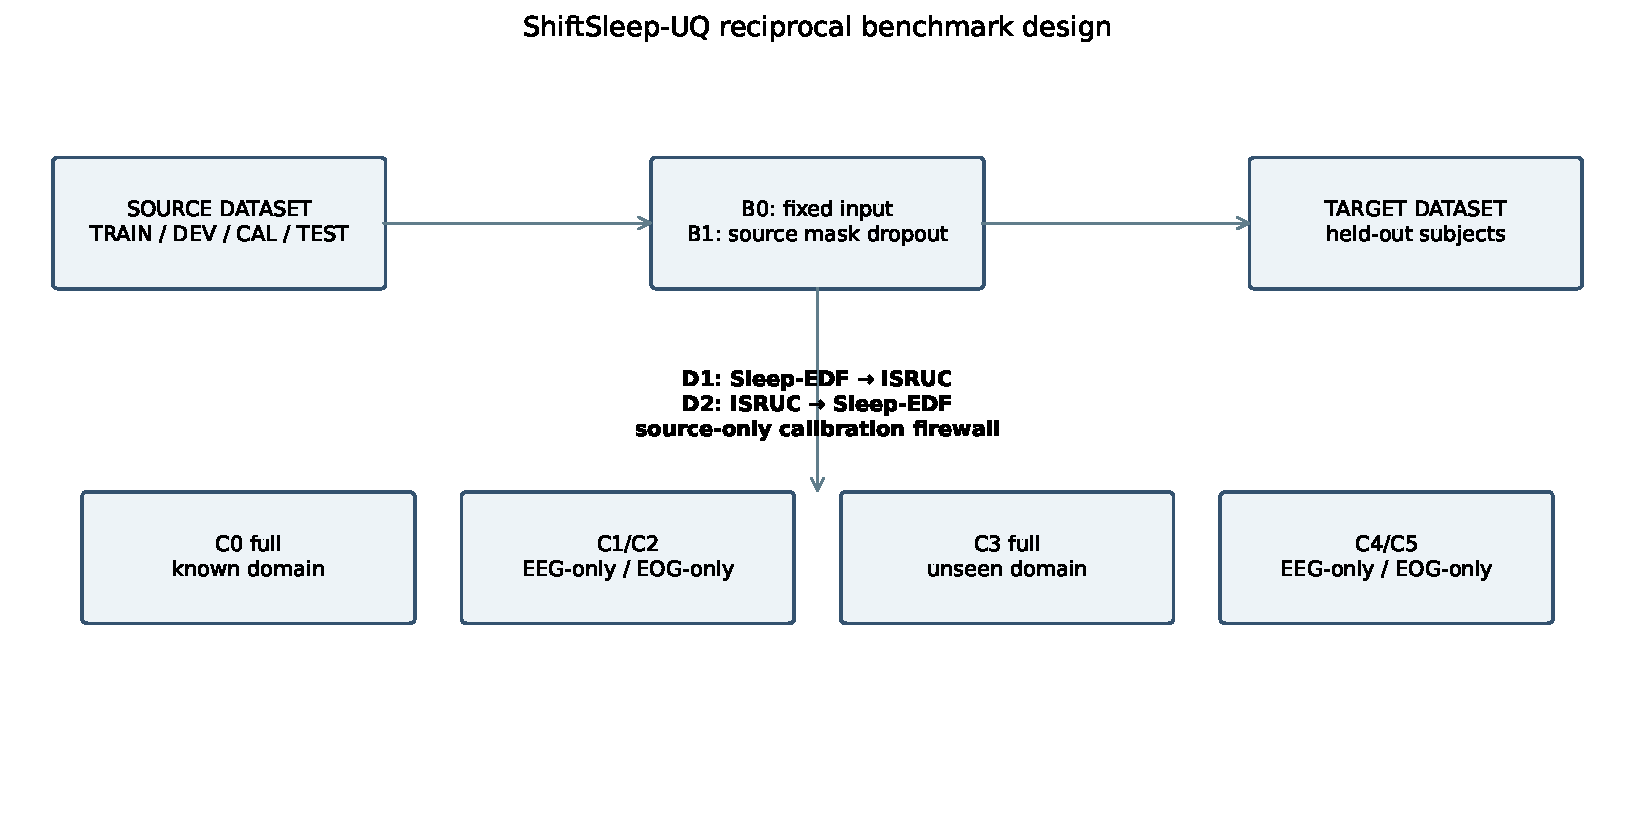
\includegraphics[width=0.9\linewidth,height=0.70\textheight,keepaspectratio]{figures/fig1_shift_design_v2.pdf}\caption{Benchmark design and factorial shift conditions. The schematic shows source roles, reciprocal directions, modality masks, B0/B1 distinction, and the source-only calibration firewall.}\label{fig:design}\end{figure}
\begin{figure}[p]\centering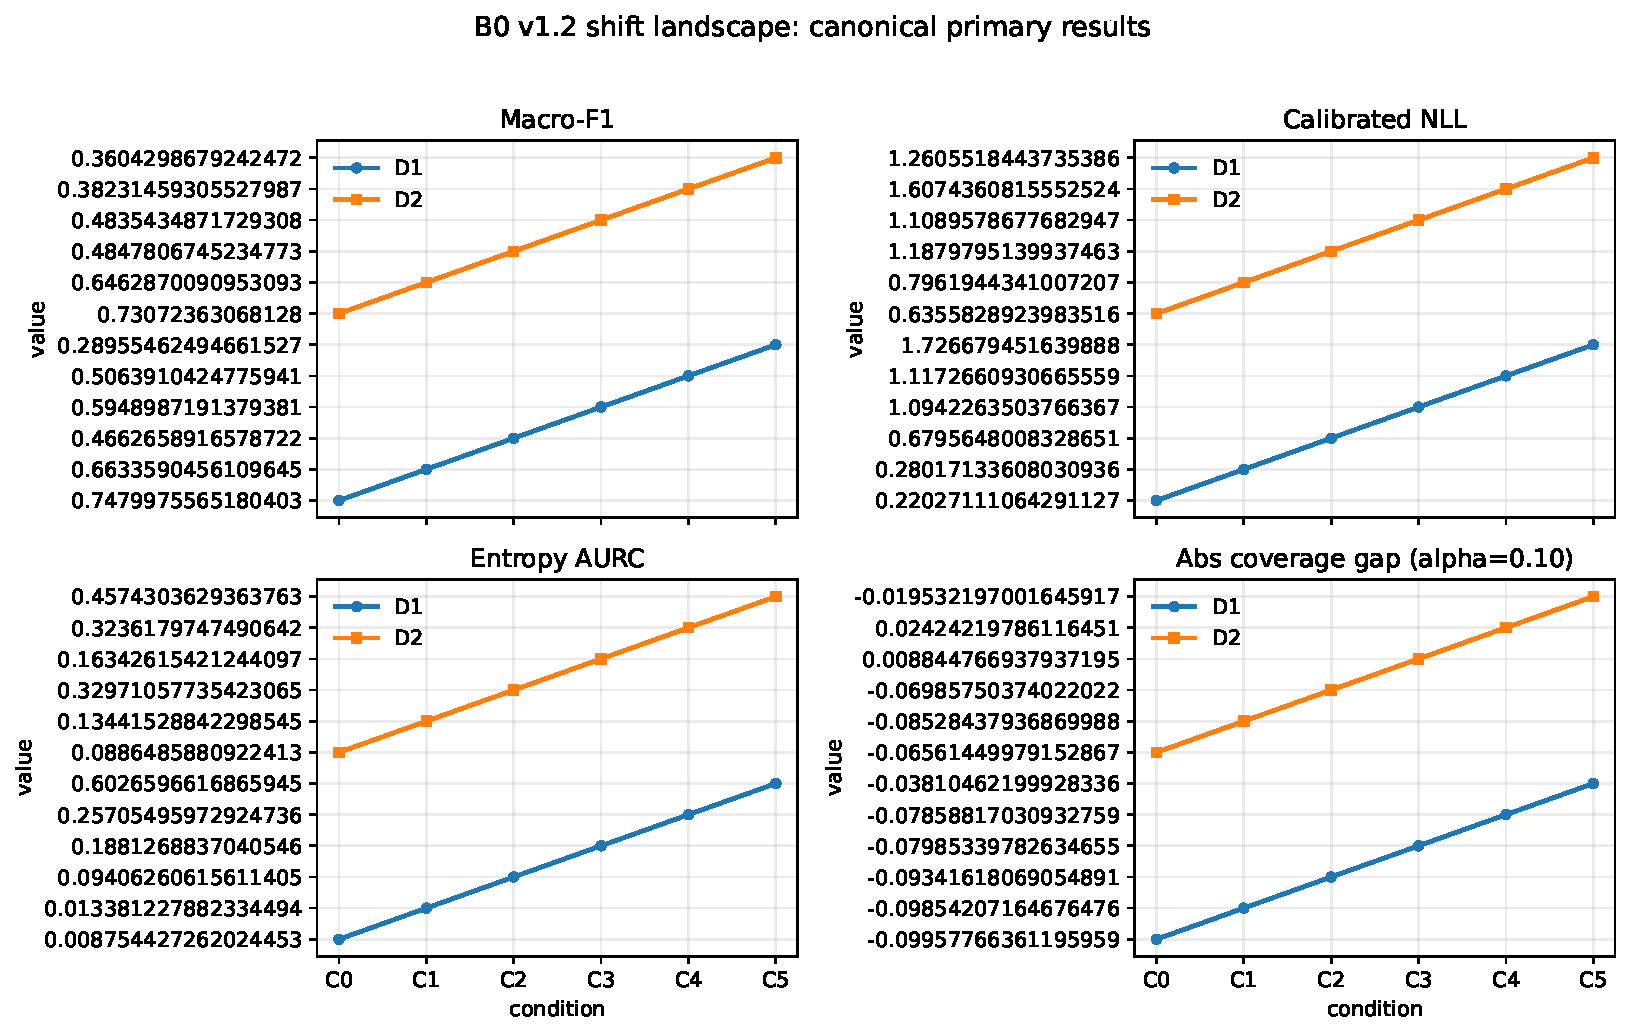
\includegraphics[width=0.9\linewidth,height=0.70\textheight,keepaspectratio]{figures/fig2_b0_shift_landscape_v2.pdf}\caption{Canonical B0 v1.2 primary results across C0--C5. This manuscript-specific rendering replaces the earlier frozen presentation because its source-data audit found the original macro-F1 panel unavailable in the figure source.}\label{fig:b0}\end{figure}
\begin{figure}[p]\centering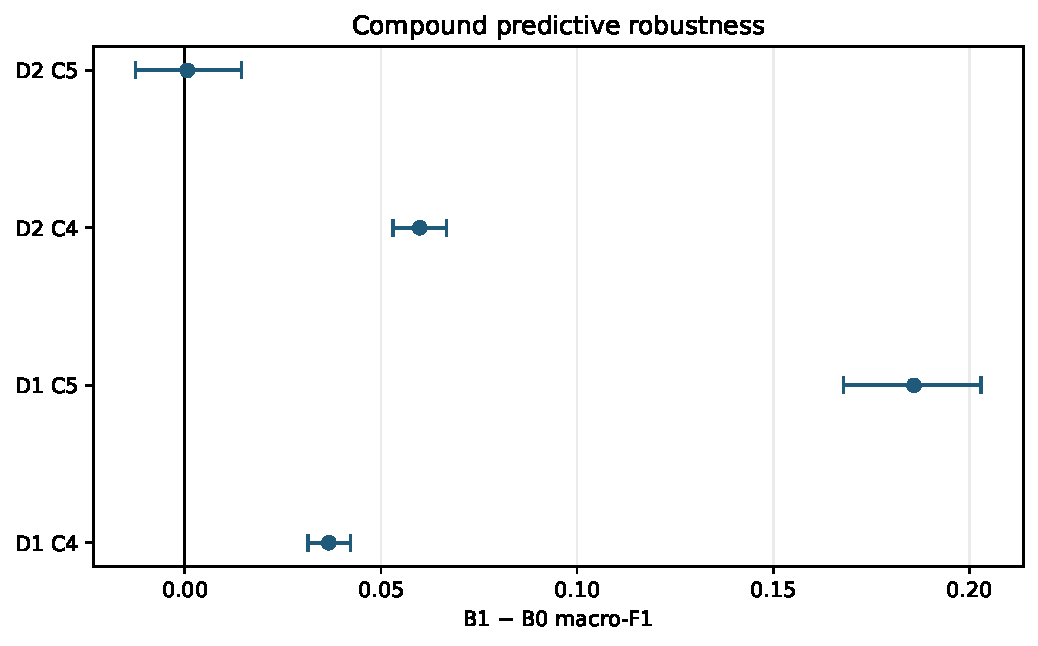
\includegraphics[width=0.9\linewidth,height=0.70\textheight,keepaspectratio]{../reports/paper_figures/figures/fig3_b1_compound_macro_f1.pdf}\caption{Paired B1--B0 macro-F1 effects in the four primary compound cells.}\label{fig:b1}\end{figure}
\begin{figure}[p]\centering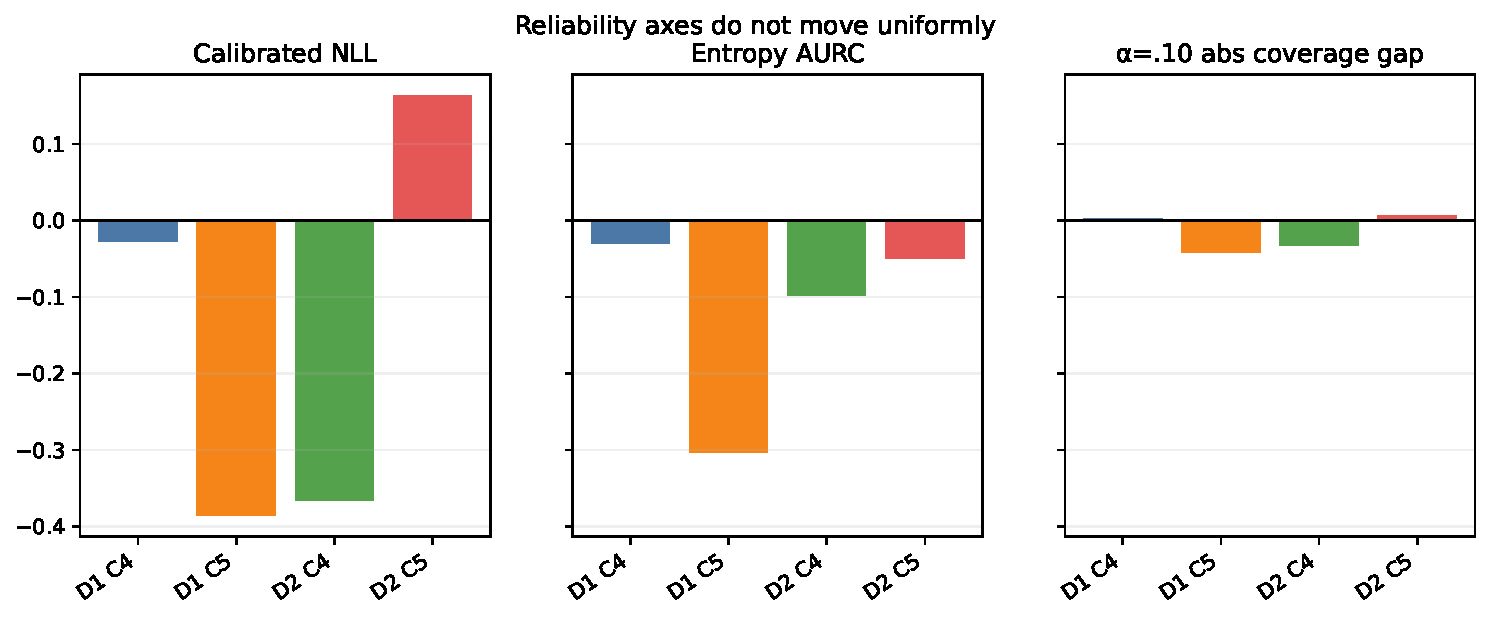
\includegraphics[width=0.9\linewidth,height=0.70\textheight,keepaspectratio]{../reports/paper_figures/figures/fig4_compound_reliability_axes.pdf}\caption{Paired effects across reliability axes.}\label{fig:rel}\end{figure}
\begin{figure}[p]\centering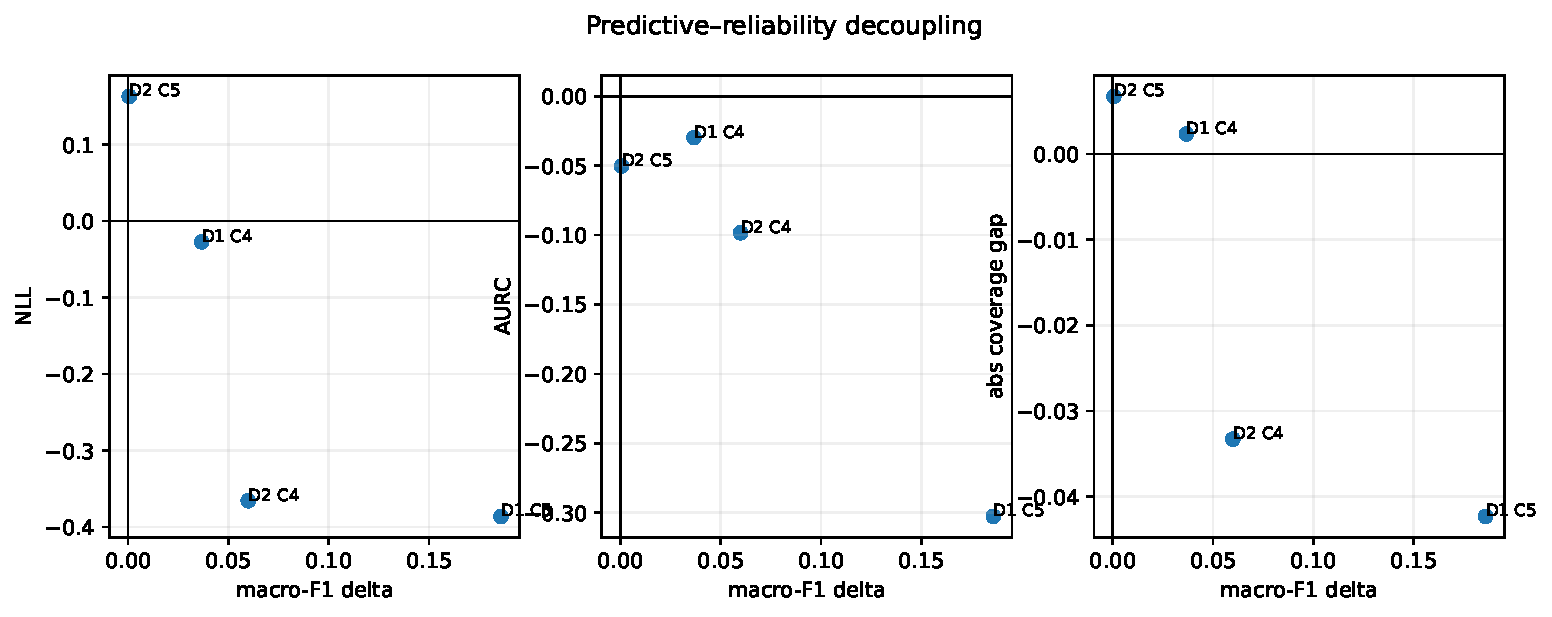
\includegraphics[width=0.9\linewidth,height=0.70\textheight,keepaspectratio]{../reports/paper_figures/figures/fig5_prediction_reliability_decoupling.pdf}\caption{Descriptive relationship between predictive and reliability changes.}\label{fig:decouple}\end{figure}
\begin{figure}[p]\centering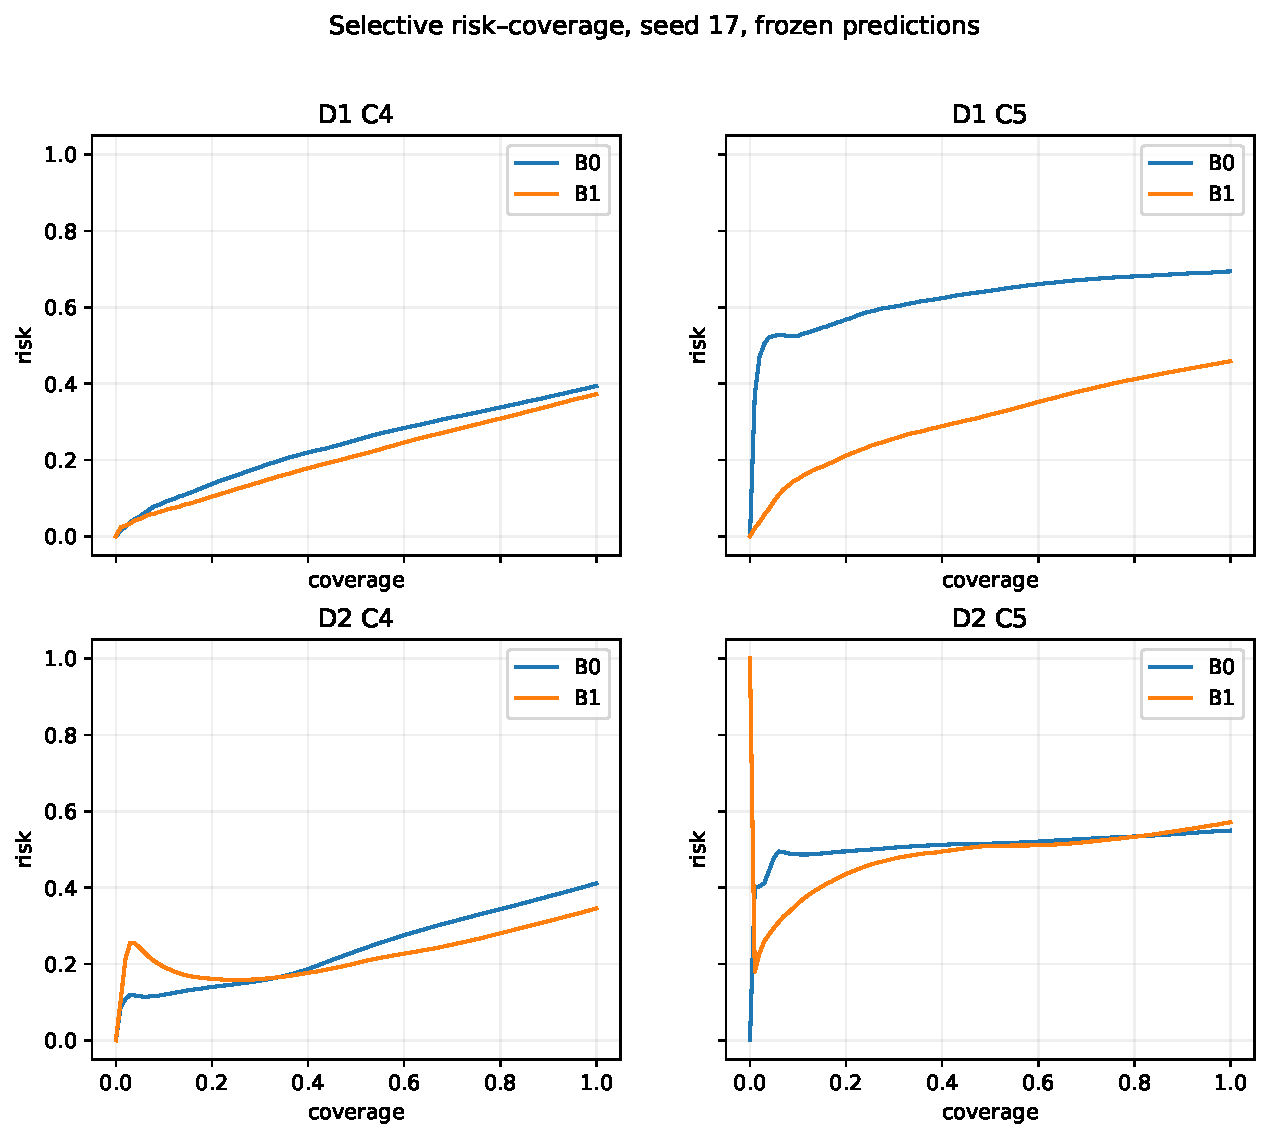
\includegraphics[width=0.9\linewidth,height=0.70\textheight,keepaspectratio]{../reports/paper_figures/figures/fig6_selective_risk_coverage.pdf}\caption{Representative frozen risk-coverage curves.}\label{fig:selective}\end{figure}
\begin{figure}[p]\centering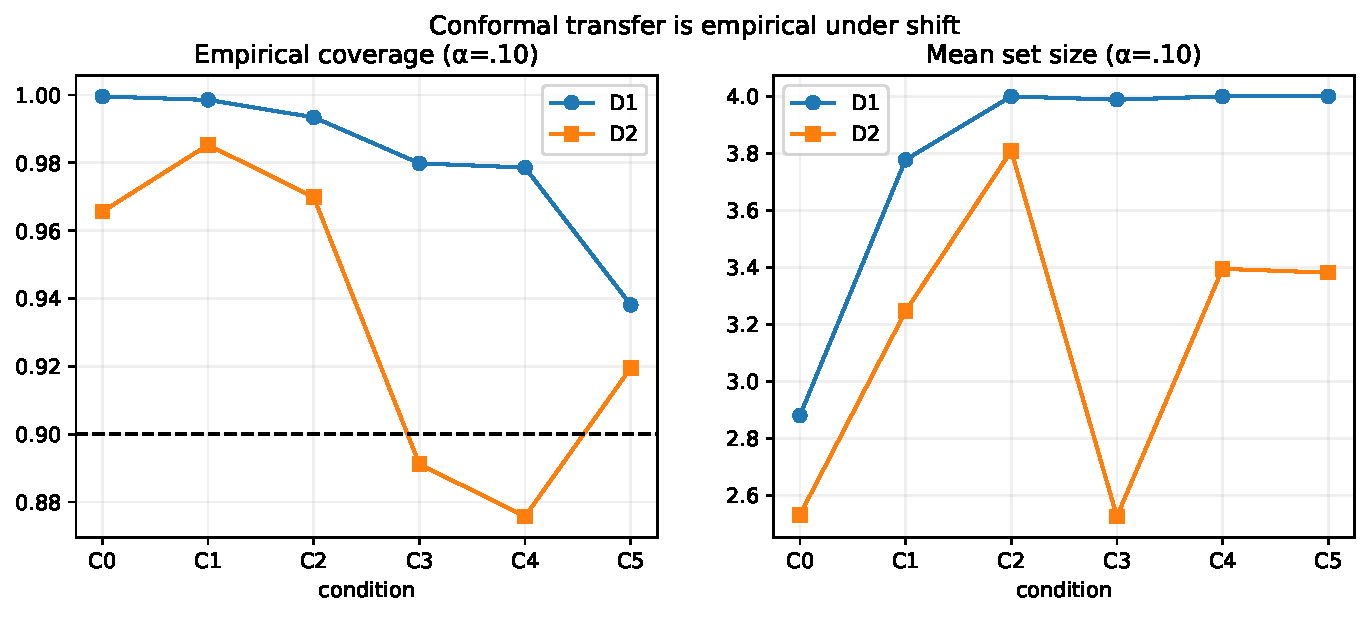
\includegraphics[width=0.9\linewidth,height=0.70\textheight,keepaspectratio]{../reports/paper_figures/figures/fig7_conformal_transfer.pdf}\caption{Empirical conformal coverage and mean set size under transfer.}\label{fig:conformal}\end{figure}
\begin{figure}[p]\centering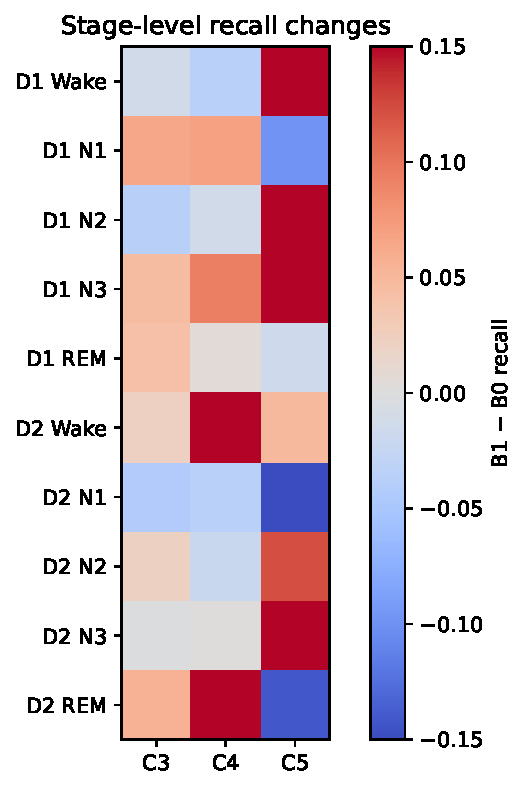
\includegraphics[width=0.9\linewidth,height=0.70\textheight,keepaspectratio]{../reports/paper_figures/figures/fig8_stage_recall_changes.pdf}\caption{Stage-level B1--B0 recall changes.}\label{fig:stage}\end{figure}
\end{document}
